\documentclass[oribibl]{llncs}
\usepackage[utf8]{inputenc}

\title{Lightweight and Accurate Memory Allocation in Key-value Cache}
% \author{Ivar Ekeland\inst{1} \and Roger Temam\inst{2}}

% \institute{Princeton University, Princeton NJ 08544, USA
% \and
% Universit\'{e} de Paris-Sud,
% Laboratoire d'Analyse Num\'{e}rique, B\^{a}timent 425,\\
% F-91405 Orsay Cedex, France}

\usepackage{graphicx}


\begin{document}

\maketitle

\begin{abstract}
The use of key-value caches in modern web servers is becoming more and more ubiquitous. Representatively, Memcached as a widely used key-value cache system, originally intended for speeding up dynamic web applications by alleviating database load. One of the key factors affecting the performance of Memcached is the memory allocation among different item classes. How to spend as little space and time as possible to obtain the most efficient partitioning scheme is the focus of attention.

One earlier study on optimizing memory allocation is LAMA, which uses footprint-based MRC to optimize memory allocation in Memcached.
\end{abstract}

\section{Introduction}
There is a theory which states that if ever anyone discovers exactly what the Universe is for and why it is here, it will instantly disappear and be replaced by something even more bizarre and inexplicable.
There is another theory which states that this has already happened.

% \begin{figure}[h!]
% \centering
% 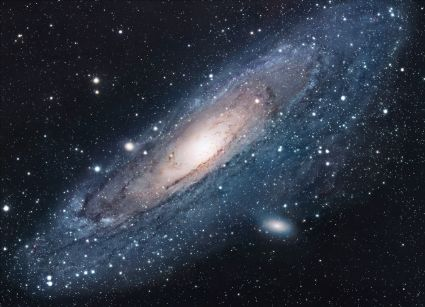
\includegraphics[scale=1.7]{universe}
% \caption{The Universe}
% \label{fig:universe}
% \end{figure}

\section{Conclusion}
``I always thought something was fundamentally wrong with the universe'' \cite{adams1995hitchhiker}

\bibliographystyle{splncs03}
\bibliography{references}
\end{document}
